\documentclass{article}

\usepackage{fancyhdr}
\usepackage{graphicx}
\usepackage{float}
\usepackage{geometry}
\geometry{margin=1in}
\setlength{\headheight}{49.4pt}
\pagestyle{fancy}
\fancyhf{}
\rhead{
    \centering
  \begin{tabular*}{\textwidth}{@{\extracolsep{\fill}}ccc}
    \small University of Florida & \textbf{\small EEL3111C - Circuits} & \small Rottenberg, Cole Harrison\\
    \small Electrical \& Computer Engineering Dept. & \small Lab 9: Filters & \small Class \#: 20931 \\
    \small Page \thepage & \small Revision: 0 & \small \today \\
  \end{tabular*}
}

\begin{document}
% I need a bold horizontal line

\begin{center}
    \hrule
    \vspace{0.2cm}
    \textbf{\large REQUIREMENTS NOT MET}
    \vspace{0.2cm}
    \hrule
\end{center}
% Bullet points on what was not met
\begin{itemize}
    \item \textbf{Requirement 1:} The final Breadboard implementation was not met due to a missing $0.1 \mu F$ capacitor. A $0.01\mu F$ capacitor was used instead to demonstrate ability.
\end{itemize}

\begin{center}
    \hrule
    \vspace{0.2cm}
    \textbf{\large PROBLEMS ENCOUNTERED}
    \vspace{0.2cm}
    \hrule
\end{center}
% More Bullet points with filler text
\begin{itemize}
    \item \textbf{Problem 1:} Missing capacitor mentioned above...
\end{itemize}

\begin{center}
    \hrule
    \vspace{0.2cm}
    \textbf{\large INTRODUCTION}
    \vspace{0.2cm}
    \hrule
\end{center}

Now we start our introduction to our write up
For your write up, write a brief introduction to what you are doing in the in lab. two to four sentences. 
Omit this section for the prelab.


\begin{center}
    \hrule
    \vspace{0.2cm}
    \textbf{\large DISCUSSION}
    % A horizontal line here
    \vspace{0.2cm}
    \hrule
\end{center}

\textbf{\large 9.5 Pre-Lab Requirements:}

\textbf{9.5.1 LTSpice Simulations:}
\begin{enumerate}
    \item Review AC Analysis in LTSpice
    \item Build a simple lowpass filter, Figure 9.2a, but set R = 10 k Ohm and C =
    0.001 $\mu F$. Set the voltage source to an AC amplitude of 1 and run an AC
    analysis with the following settings: Decade, 100, 1, 1Meg. Save an image of
    the circuit, a plot of the output, and table the 3 dB frequency for submission.
    \begin{figure}[H]
        \centering
        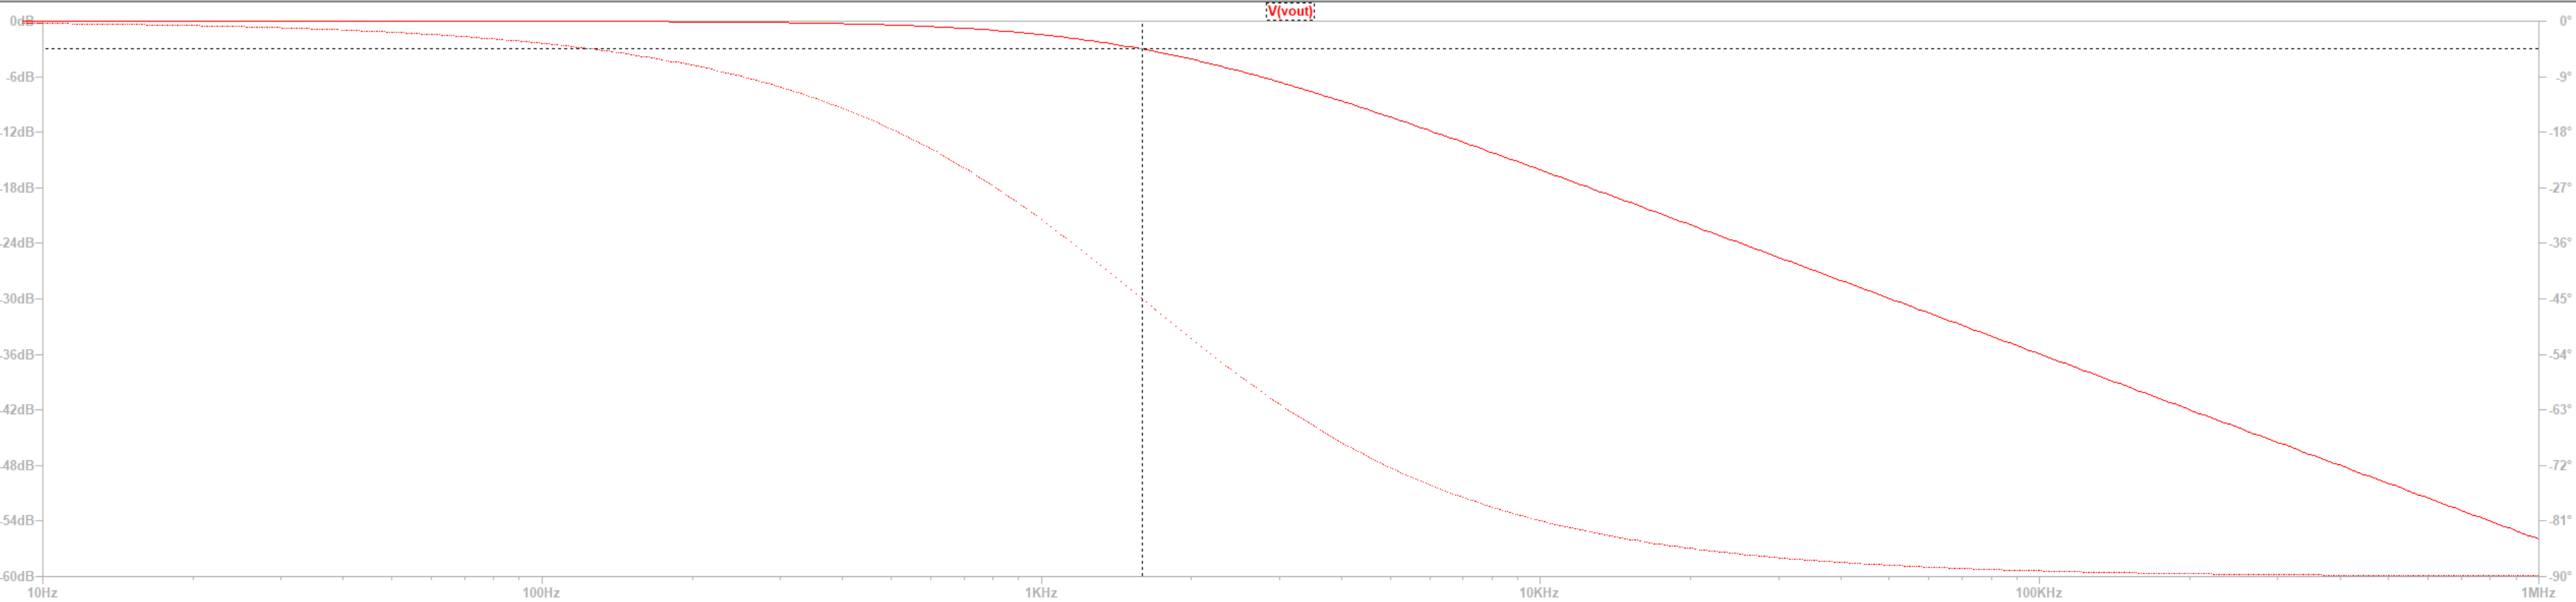
\includegraphics[width=0.5\textwidth]{2simPlot.png}
        \caption{Plot of Low Pass Filter}
    \end{figure}
    \begin{figure}[H]
        \centering
        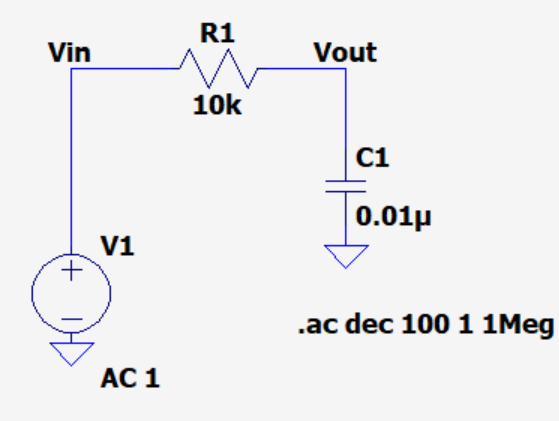
\includegraphics[width=0.5\textwidth]{2simCircuit.png}
        \caption{Circuit of Low Pass Filter}
    \end{figure}
    \begin{tabular}{|c|c|c|}
        \hline
        LOW-PASS & 1.6 kHz & $45\deg$ \\
        \hline
        \end{tabular}
    \item High Pass Filter
    \begin{figure}[H]
        \centering
        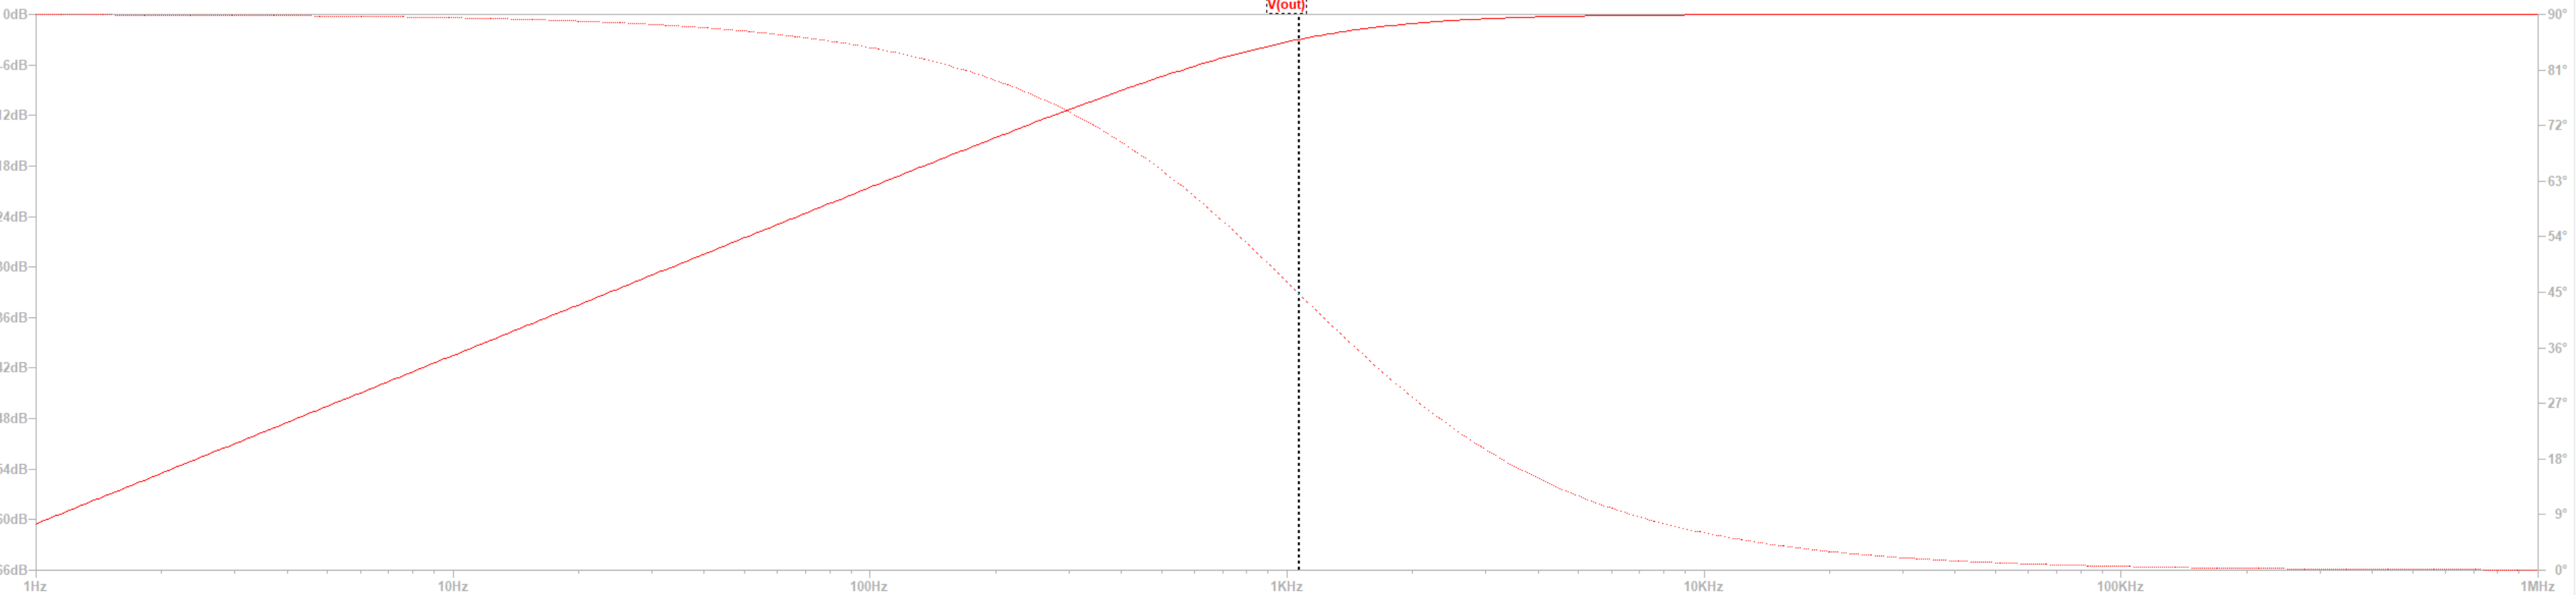
\includegraphics[width=0.5\textwidth]{3simPlot.png}
        \caption{Plot of High Pass Filter}
    \end{figure}
    \begin{figure}[H]
        \centering
        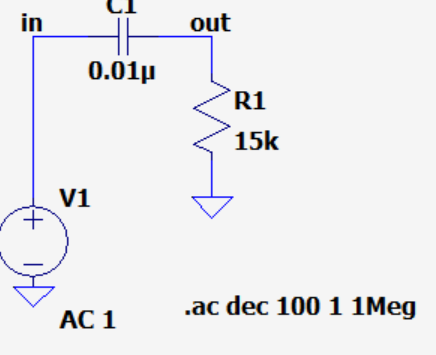
\includegraphics[width=0.5\textwidth]{3simCircuit.png}
        \caption{Circuit of High Pass Filter}
    \end{figure}
    \begin{tabular}{|c|c|c|}
        \hline
        HIGH-PASS & 1.063 kHz & $45\deg$ \\
        \hline
        \end{tabular}
    \item Active Low Pass Filter with $R = 1k \Omega$ and $C = 0.1 \mu F$
    \begin{figure}[H]
        \centering
        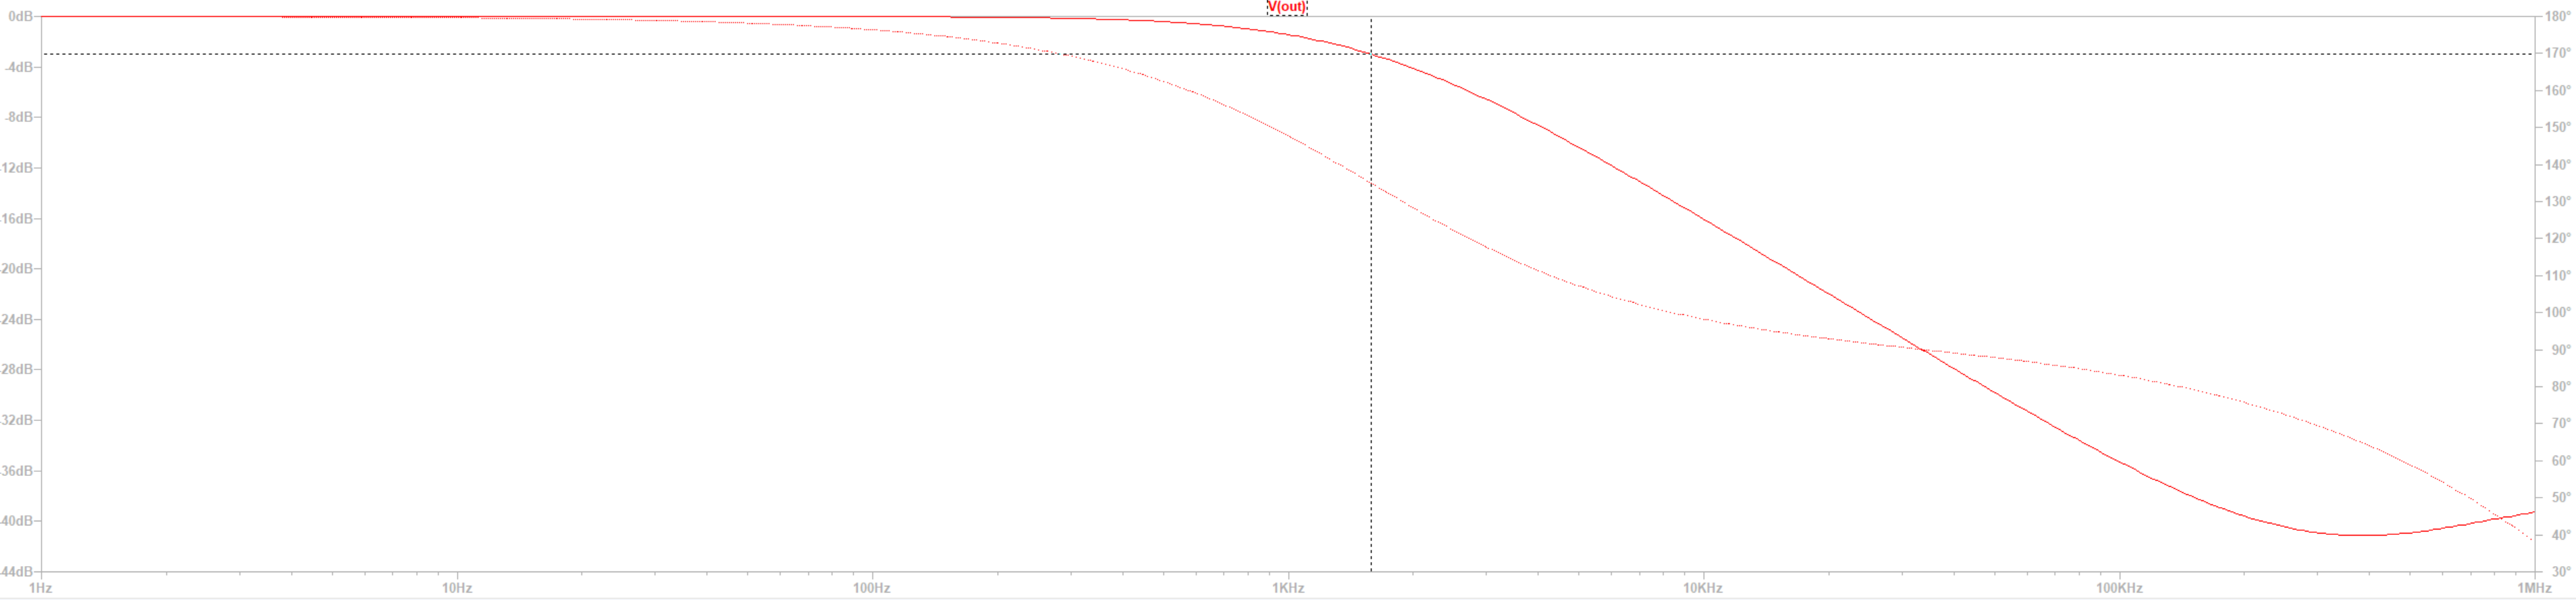
\includegraphics[width=0.5\textwidth]{4simPlot.png}
        \caption{Plot of Active Low Pass Filter}
    \end{figure}
    \begin{figure}[H]
        \centering
        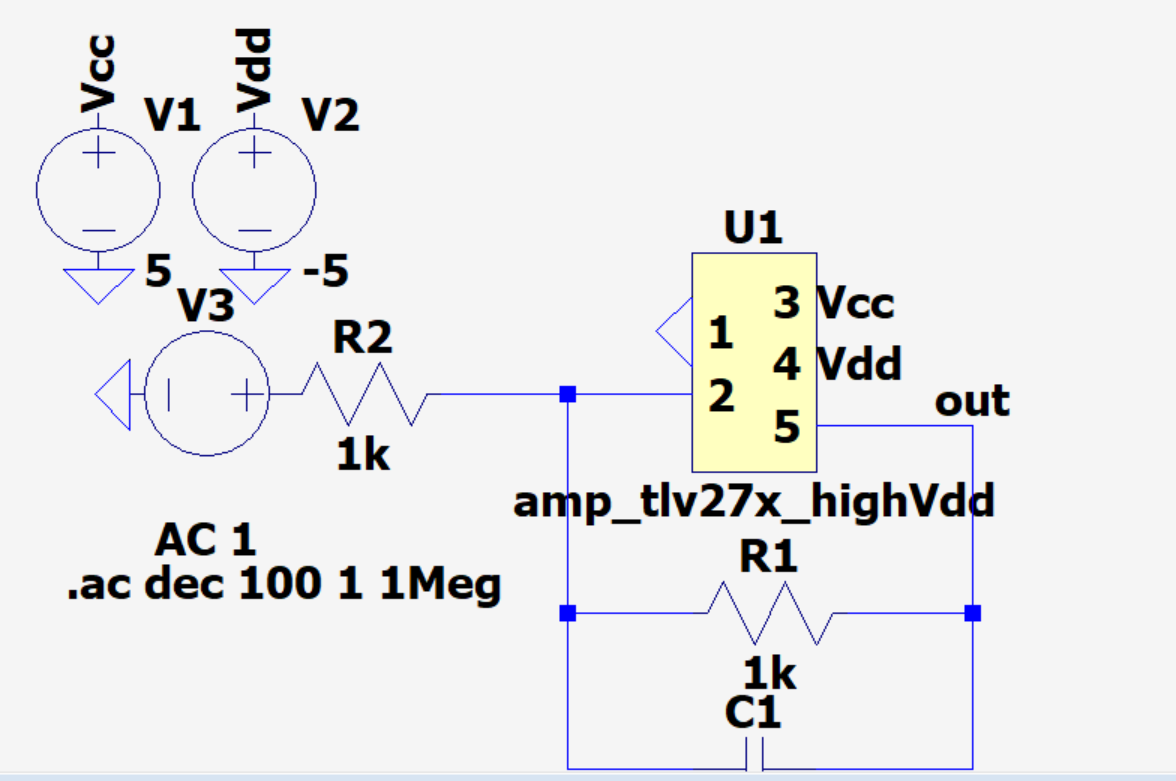
\includegraphics[width=0.5\textwidth]{4simCircuit.png}
        \caption{Circuit of Active Low Pass Filter}
    \end{figure}
    \begin{tabular}{|c|c|c|}
        \hline
        ACTIVE LOW-PASS & 1.59 kHz & $45\deg$ \\
        \hline
        \end{tabular}
    \item Active High Pass Filter with $R_1 = 3.3k \Omega, R_2 = 33k \Omega$ and $C = 0.1 \mu F$
    \begin{figure}[H]
        \centering
        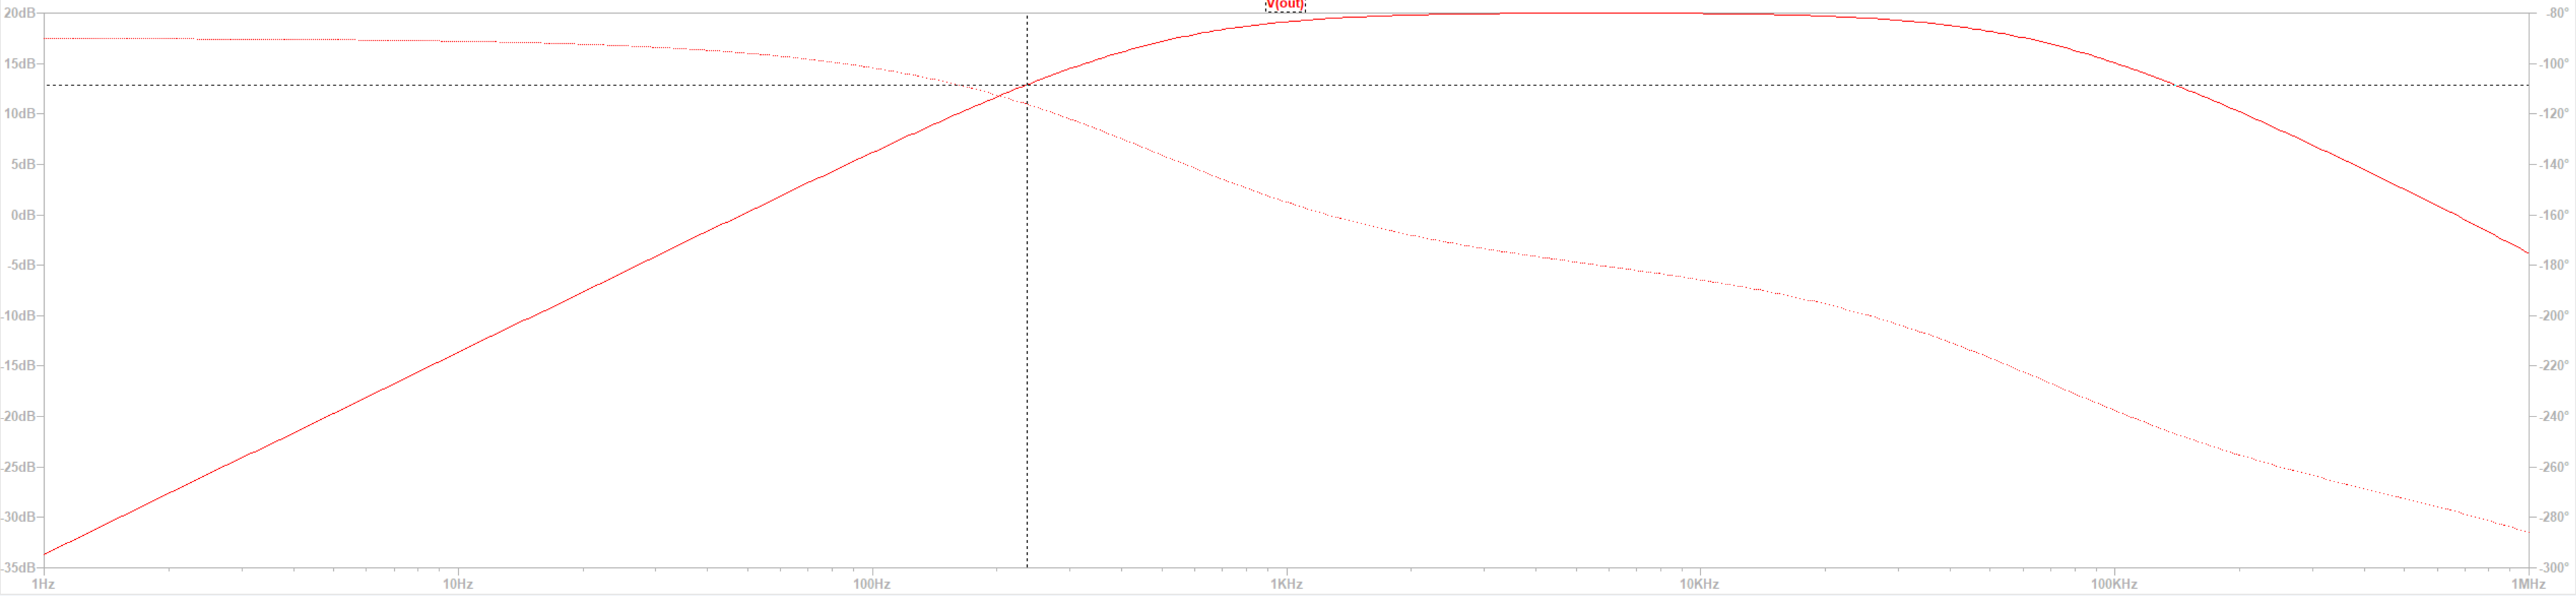
\includegraphics[width=0.5\textwidth]{5simPlot.png}
        \caption{Plot of Active High Pass Filter}
    \end{figure}
    \begin{figure}[H]
        \centering
        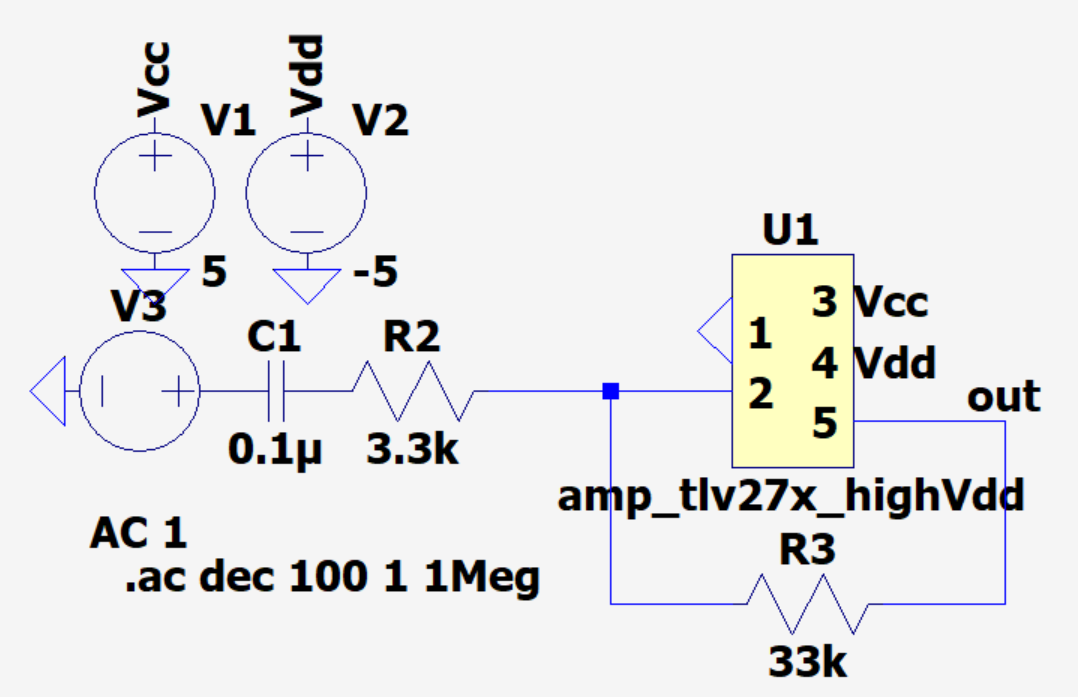
\includegraphics[width=0.5\textwidth]{5simCircuit.png}
        \caption{Circuit of Active High Pass Filter}
    \end{figure}
    \begin{tabular}{|c|c|c|}
        \hline
        ACTIVE HIGH-PASS & 482.3 Hz & $45\deg$ \\
        \hline
        \end{tabular}
\end{enumerate}
\textbf{9.5.2 Breadboard Implementation:}
\begin{enumerate}
    \item Review Network Analyzer tool in Digilent Waveforms.
    \item Build Active Low Pass Filter with $R = 1k \Omega$ and $C = 0.1 \mu F$.
    \item Network Analysis of Circuit
    \begin{figure}[H]
        \centering
        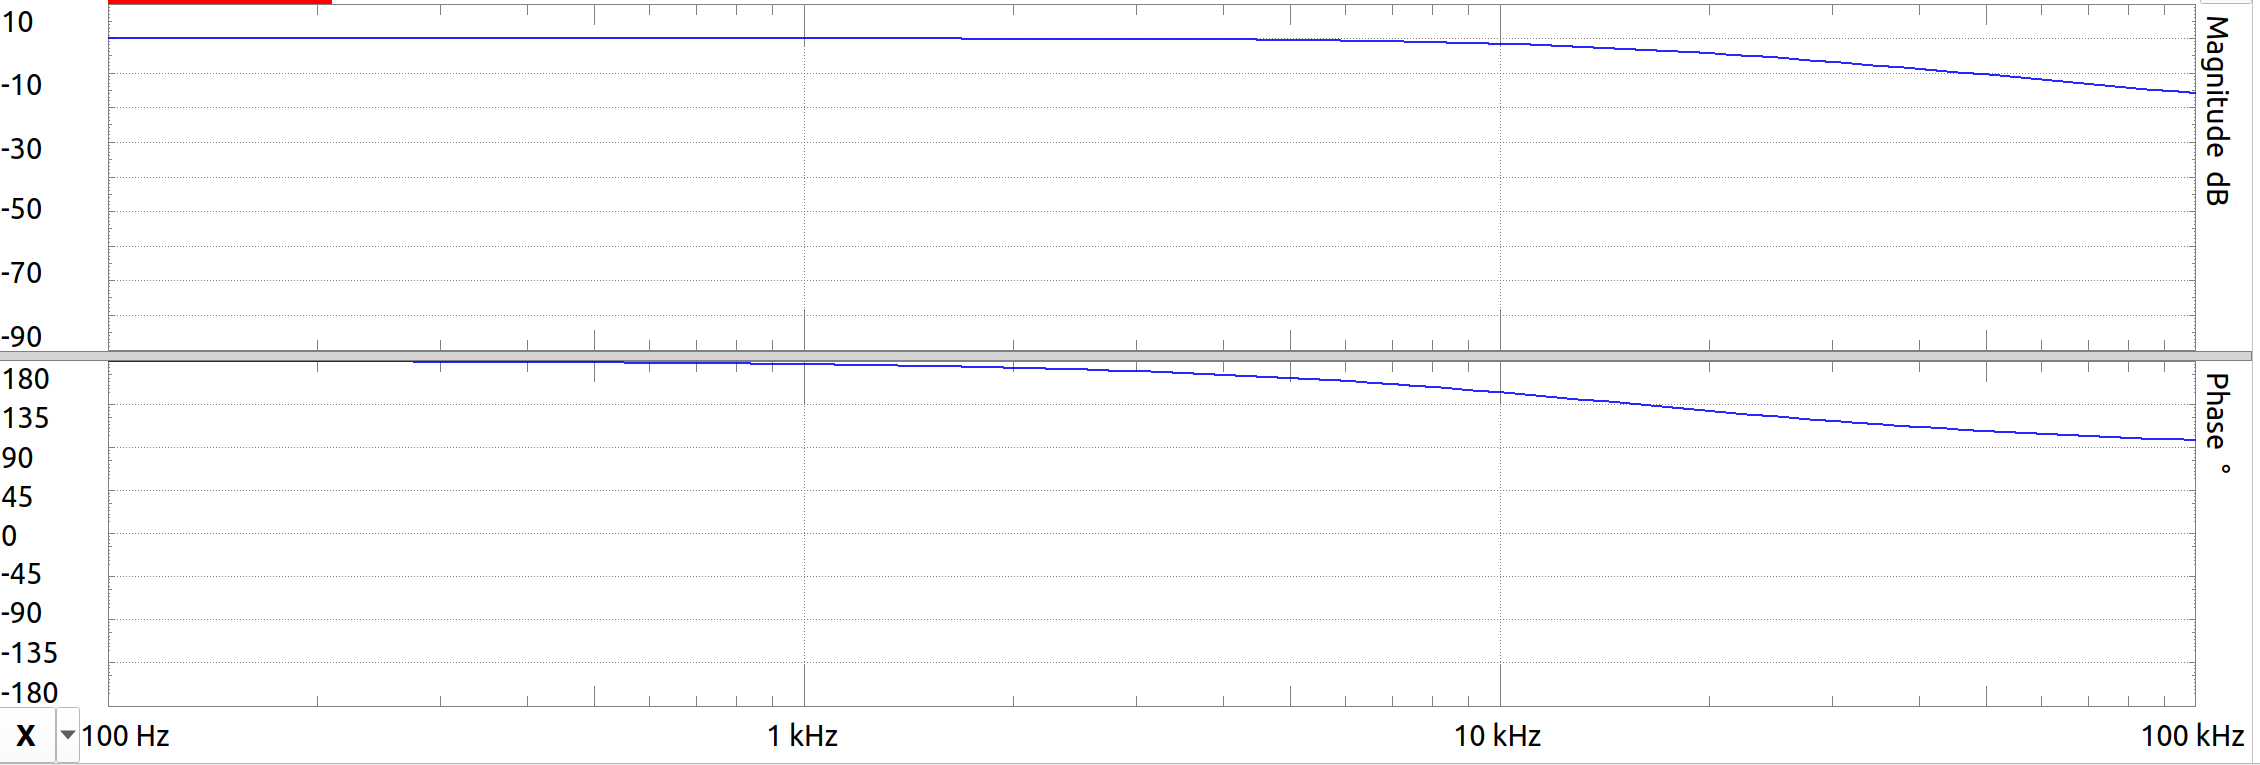
\includegraphics[width=0.5\textwidth]{3physPlot.png}
        \caption{Plot of Active Low Pass Filter}
    \end{figure}
\end{enumerate}
\texfbf{\large9.6 In-Lab Requirements:}
Finished.

\texfbf{\large9.7 Write-Up:}

\begin{center}
    \hrule
    \vspace{0.2cm}
    \textbf{\large CONCLUSION}
    % A horizontal line here
    \vspace{0.2cm}
    \hrule
\end{center}

This is where I start to answer the questions in the lab. We only need to do this for the write up.

\end{document}